\chapter{Introduction to Fracture Mechanics} \label{chap:app-intro-fracture}

Fracture mechanics is the study of how cracks propagate through materials and is of critical importance in types of engineering where machines and structures are subjected to varying loads, or are subjected to loads causing substantial yielding.
When cracks are present, structures run the risk of sudden failure, even if the nominal stresses in the cracked region are substantially below the ultimate strength of the material.
One goal of fracture mechanics is to predict how cracks will grow over time (or if their size will remain constant), which can be used to schedule inspection of critical components, or to estimate the components' safe service life (if the components cannot be inspected).

Fracture mechanics is a critical part of safe design in aerospace applications.
Where many engineering applications can avoid considering fracture by simply increasing factors of safety and adding additional material, aerospace components must be as lightweight as possible.
For components subjected to loads that do not cause significant yielding, a linear elastic material model is used.
This model assumes that crack growth is largely determined by a stress intensity factor \K, and that a very small region at the crack boundary has exceeded the yield strength and undergone plastic deformation.
For components subjected to larger loads, an elastic-plastic material model is used.
This model assumes that crack growth is largely determined by calculating a contour integral \J that corresponds to the strain energy released during crack extension, and that a much larger region near the crack boundary has undergone plastic deformation.
\J also characterizes the stress and strain state at the crack tip.
Both \K and \J are defined in later sections of this dissertation, and are important parameters not only for this research, but throughout fracture mechanics.

\section{Basics of Fracture Mechanics}

In the early twentieth century, theories of fracture mechanics were limited to brittle materials like glass.
Alan A. Griffith theorized that cracks in brittle materials extended whenever the energy required to break atomic bonds to form new crack surfaces was less than the strain energy created by applied loads.
As tensile loads are applied to a body, the strain energy in the body increases.
As the crack extends, energy is consumed as atomic bonds are broken.
The total potential energy (\(\Pi\))\nomenclature[2\Pi]{\(\Pi\)}{total potential energy} in the cracked body decreases as the crack extends.
In the years following World War II, George R. Irwin extended this energy balance method to include energy consumed by yielding of the material in the region near the crack tip.
Irwin defined a strain energy release rate \nomenclature[1G]{\G}{strain energy release rate with respect to crack size}\G related to changes in crack size and a correlated stress intensity factor \nomenclature[1K]{\K}{linear elastic stress intensity factor}\K.
For through cracks with length \(2a\) \nomenclature[1a]{\(a\)}{half crack length for through cracks} in an infinite plate with remote tensile stress \St\nomenclature[2\sigma_t]{\St}{applied tensile stress}. shown in \Cref{fig:through-crack-infinite-plate},
  \begin{align}
    \G &= - \frac{d \Pi}{dA} = \frac{\pi \St^2 a}{E'} = \frac{\KI^2}{E'} \label{eq:g} \\
    \intertext{where}
    A &= 2at = \textnormal{area of cracked surfaces} \\
    E' &=
    \begin{cases}
      E & \textnormal{for plane stress} \\
      \frac{E}{(1-\nu^2)} & \textnormal{for plane strain}
    \end{cases} \\
    \KI &= \St \sqrt{\pi a}.
  \end{align}
\begin{figure}[tbp]
\centering
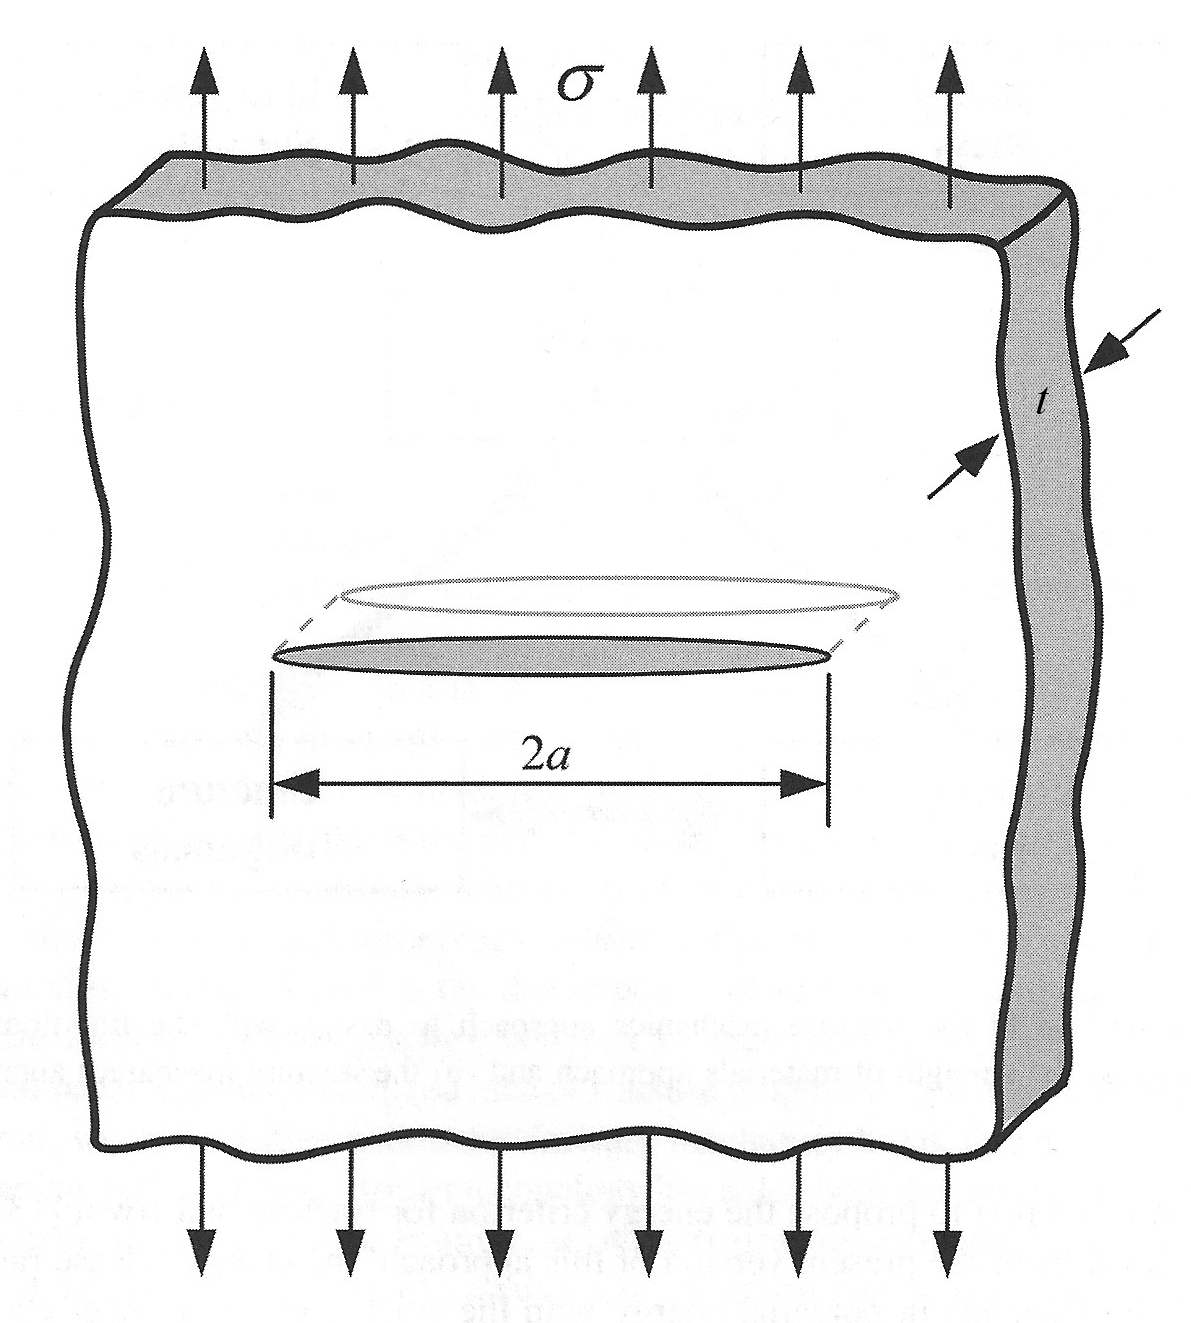
\includegraphics[width=0.5\columnwidth]{through-crack-infinite-plate}
\caption[A through crack in an infinite plate loaded in tension]{A through crack in an infinite plate loaded in tension \citep{anderson2005} \label{fig:through-crack-infinite-plate}}
\end{figure}

If a polar coordinate system is established at the crack tip, with \(\theta=0\)\nomenclature[2\theta]{\(\theta\)}{angle from crack plane} corresponding to the crack plane, the normal stresses (\Sxx\nomenclature[2\sigma_xx]{\Sxx}{normal stress, $x$ direction} and \Syy\nomenclature[2\sigma_yy]{\Syy}{normal stress, $y$ direction}) and principal stresses (\Sone\nomenclature[2\sigma_1]{\Sone}{first principal stress} and \Stwo\nomenclature[2\sigma_2]{\Stwo}{second principal stress}) at a distance \(r\)\nomenclature[1r]{\(r\)}{radial distance from the crack tip} ahead of the crack tip are identical
\begin{align}
\Sxx(r,0) &= \Syy(r,0) = \Sone(r,0) = \Stwo(r,0) = \frac{\KI}{\sqrt{2\pi r}} \label{eq:singularity}
\end{align}
and \(\Sxx = \Syy = \Sone = \Stwo = \infty\) at \(r=0\).
Because infinite stress values are unrealistic, stress values near the crack are limited to the material yield stress \Sys\nomenclature[2\sigma_ys]{\Sys}{material yield stress}.
This limit occurs at all points \(r<\ry\), where \ry\nomenclature[1ry]{\ry}{first order estimate of plastic zone radius} is defined as
  \begin{align}
  \ry &=
    \begin{cases}
      \frac{1}{2\pi} \left( \frac{\KI}{\Sys} \right)^2 & \textnormal{for plane stress} \\
      \frac{1}{6\pi} \left( \frac{\KI}{\Sys} \right)^2 & \textnormal{for plane strain.} \\
    \end{cases} \label{eq:ry}
  \end{align}
Because changing the upper limit of stress changes the force equilibrium in the body, the additional stress is redistributed into the uncracked region.
This redistribution leads to the definition of a plastic zone size \rp\nomenclature[1rp]{\rp}{second order estimate of plastic zone radius}
\begin{align}
  \rp &=
    \begin{cases}
      \frac{1}{\pi} \left( \frac{\KI}{\Sys} \right)^2 & \textnormal{for plane stress} \\
      \frac{1}{3\pi} \left( \frac{\KI}{\Sys} \right)^2 & \textnormal{for plane strain.}
    \end{cases} \label{eq:rp}
\end{align}
The material in the plastic zone carries some stress, but is weaker than the material subjected to stresses in the elastic range.
Irwin approximated the effect this has on the cracked body by defining a larger apparent crack length \aapp:
\begin{align}
\aapp &= a+\ry = a + \frac{\rp}{2}.
\end{align}
The increased crack length yields a new effective stress intensity factor \(K_{\textnormal{Iapp}}\)
\begin{align}
K_{\textnormal{Iapp}} &= \St \sqrt{\pi \aapp} \label{eq:kiapp}
\end{align}
which can be substituted into \Cref{eq:rp} to find a new plastic zone size \rp.
Repeating this process will lead to converged, corrected values for \KI and \aapp.

\section{The Surface Crack Problem}

  The proposed research will focus on surface cracks in plates loaded
  in bending by a remote bending moment \M.\nomenclature[1M]{\M}{applied bending moment}
A schematic of one such plate is shown in \Cref{fig:cracked-plate}.
The plate is \(2W\)\nomenclature[1W]{\(W\)}{half plate width} wide, 
\(t\)\nomenclature[1t]{\(t\)}{plate thickness} thick, and \(2H\)\nomenclature[1H]{\(H\)}{half plate height} high.
The plate has a semi-elliptical crack on its front surface.
The crack is \(2c\)\nomenclature[1c]{\(c\)}{half crack width for surface cracks} wide, and extends a distance \(a\)\nomenclature[1a]{\(a\)}{crack depth for surface cracks} into the plate.
Any position \((x_\textnormal{e}, y_\textnormal{e})\)\nomenclature[1xe]{\(x_\textnormal{e}\)}{horizontal coordinate of point along front of semi-elliptical surface crack}\nomenclature[1ye]{\(y_\textnormal{e}\)}{vertical coordinate of point along front of semi-elliptical surface crack} along the elliptical crack front can be defined in terms of an angle \(\phi\)\nomenclature[2\phi]{\(\phi\)}{parametric angle defining position along crack front} along a circle defined by points (\(x_\textnormal{c}, y_\textnormal{c}\))\nomenclature[1xc]{\(x_\textnormal{c}\)}{horizontal coordinate of point along circle inscribed in semi-elliptical surface crack}\nomenclature[1yc]{\(y_\textnormal{c}\)}{vertical coordinate of point along circle inscribed in semi-elliptical surface crack} centered within the crack with radius \(a\)
\begin{align*}
      y_\textnormal{c} &= y_\textnormal{e} = a \sin \phi \\
      x_\textnormal{c} &= \sqrt{ a^2 - y_\textnormal{e}^2 } = a \cos \phi \\
      x_\textnormal{e} &= c \cos \phi \\
                  \phi &= \arctan \frac{y_\textnormal{c}}{x_\textnormal{c}} .\\
\end{align*}
  \begin{figure}[tbp]
  \centering
    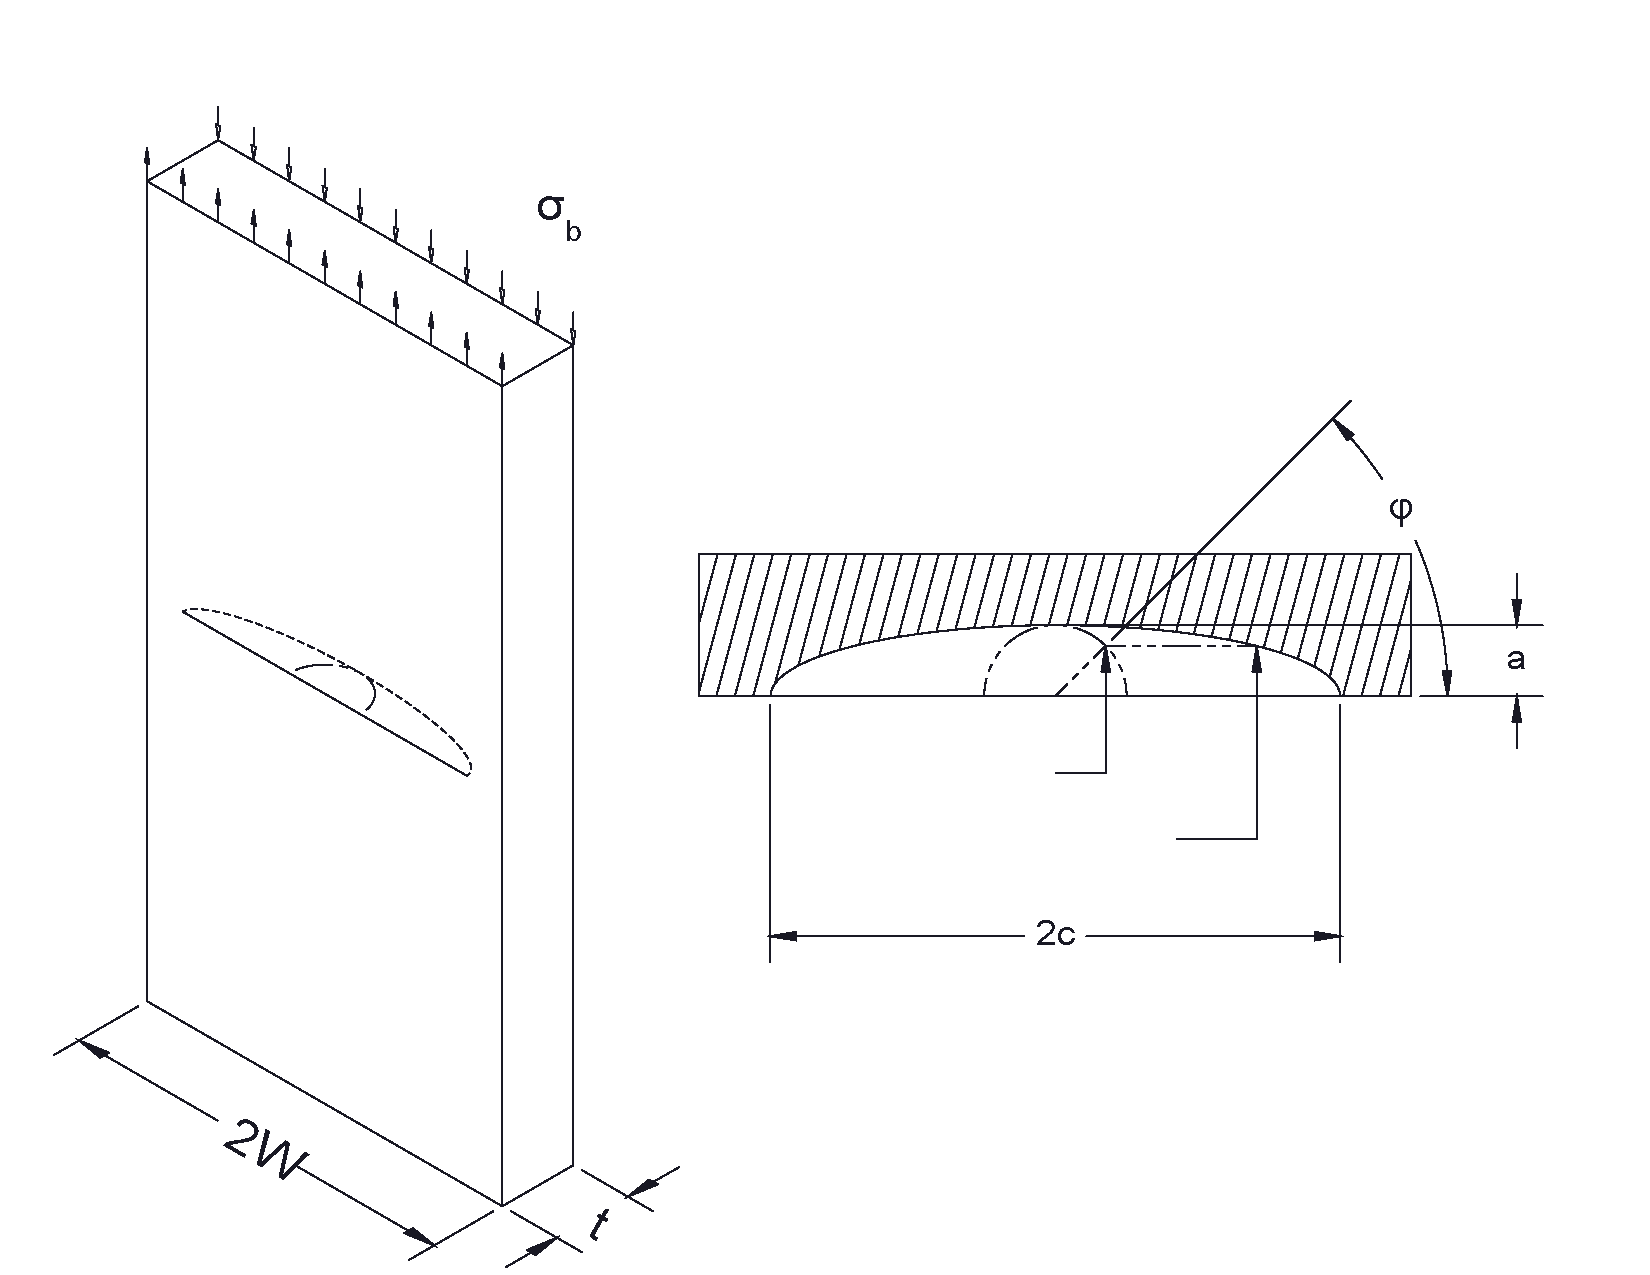
\includegraphics[width=0.9\columnwidth]{plate-bending-2}
    \caption{Schematic of cracked plate \label{fig:cracked-plate}}
  \end{figure}

Early research on surface cracks focused on tension loads, and shallow cracks in bending are similar to cracks in tension. \citet{greensneddon1950} found an analytical solution of stress intensity factors for an elliptical crack embedded in an infinite solid.
Since practical applications are for finite-thickness bodies, and most cracks start at a free surface, \citet{irwin1962} imagined removing a finite-thickness strip of material from the infinite solid.
One boundary of the strip bisected the elliptical crack along its major axis.
This created an analogous model of a large finite-thickness plate with a semi-elliptical surface crack.
Three rough corrections were applied to account for the effects of
\begin{enumerate}
\item the newly-created cracked free surface,
\item plastic strains increasing the effective crack size,
\item and the plate's finite thickness.
\end{enumerate}
At \(\phi= \frac{\pi}{2}\), where Sneddon calculated the highest stress intensity, the crack is in a plane strain state.
Thus, the first correction is a free surface correction factor of 1.1 for a semi-infinite edge-cracked plate analyzed in plane strain.

For the second correction, the plastic zone size in plane strain is
\[\rp = \frac{1}{4\sqrt{2}} \left(\frac{\KI}{\Sys}\right)^2, \]
and assumed to be constant along the entire crack front.
In areas away from the highest stress intensity, any increase in plastic zone size due to a more plane-stress-like state is counteracted by lower stresses near the free surface.
Irwin assumed that these factors cancel out.

The correction for finite thickness was neglected, and Irwin rationalized this simplification as only relevant when \(\frac{a}{t}\) approaches unity.
Later research would place extend Irwin's estimates to a much broader range of geometry.
Irwin's final estimate for \KI at \(\phi=\frac{\pi}{2}\) is
\begin{align}
\KI^2 &= \frac{1.2 \St^2 \pi a}{\Phi^2 - 0.212 \left(\frac{\St}{\Sys}\right)^2} \\
\KI   &= 1.1 \St \sqrt{\pi a} \left[ F \left(\frac{a}{c},\frac{\St}{\Sys}\right) \right]\\
      \intertext{where}
F\left(\frac{a}{c},\frac{\St}{\Sys}\right) &= \left[\Phi^2 - 0.212 \left(\frac{\St}{\Sys}\right)^2\right]^{-0.5} \\
\Phi &= \Int{\sqrt{\left[ \sin^2 \phi + \left(\frac{a}{c}\right)^2 \cos^2 \phi \right]}}{\phi,0,\frac{\pi}{2}}
\end{align}
for problems where \(\frac{c}{W} \ll 1\), \(\frac{a}{c} < 1\), and \(\frac{a}{t} < 0.5\).
Here, \(\Phi\)\nomenclature[2\Phi]{\(\Phi\)}{complete elliptic integral of the second kind} is the complete elliptic integral of the second kind, and \(\Phi^2\) can be approximated as
\begin{align}
\Phi^2 &= Q = 1 + 1.464 \left( \frac{a}{c} \right)^{1.65} \label{eq:shape-factor}
\end{align}
where \(Q\)\nomenclature[1Q]{\(Q\)}{ellipse shape factor} is called the shape factor of the ellipse representing the crack front.

Irwin's stress intensity factor solution corrected for both a free surface and a small plastic zone size.
However, its use was limited to for wide bodies with relatively narrow and shallow cracks, where \(c \ll W\) and \(a \ll t\).
The next three subsections discuss methods for estimating stress intensity factors for a broader range of crack sizes.

\subsection{Early Efforts to Quantify Effects of Finite Thickness}
The first attempts to account for finite thickness were based on the alternating method.
The alternating method was first published by Hermann Schwarz around 1870 \citep{schwarzbiography}, and is a method for solving partial differential equations on a domain.
The domain is split up into two overlapping subdomains, and the differential equations are solved on one subdomain.
Second, the resulting solution is used as a set of boundary conditions for solving the differential equations on the second subdomain.
Third, the solution for the second subdomain is used as a set of boundary conditions to re-solve the differential equations on the first subdomain.
The alternating solution steps are repeated until the solutions converge.

\begin{figure}[tbp]
\centering
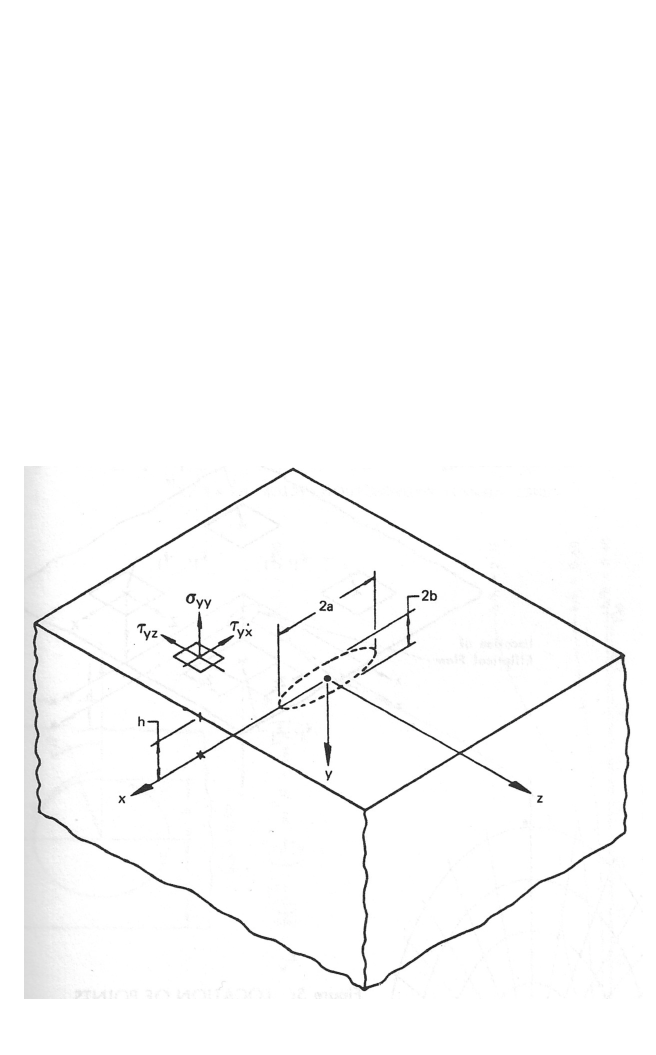
\includegraphics[width=0.8\columnwidth]{shah-semi-infinite}
\caption[Semi-infinite solid with embedded elliptical crack]{Semi-infinite solid with embedded elliptical crack \citep{shahkobayashi1972}\label{fig:shah-semi-infinite}}
\end{figure}

Two notable papers using the alternating method for surface cracks are ``On the Surface Flaw Problem'' \citep{shahkobayashi1972} for semi-ellip\-ti\-cal surface cracks and ``The Elastic Analysis of the Part-Cir\-cular Surface Flaw Problem by the Alternating Method'' \citep{smith1972} for part-cir\-cu\-lar cracks with the center of the crack located some distance from the surface.
Both papers use an infinite solid with an embedded elliptical or circular crack shown in \Cref{fig:shah-semi-infinite} as the first domain, and a semi-infi\-nite solid with the semi-ellip\-ti\-cal or semi-cir\-cu\-lar crack in the free surface as the second domain.
Shah and Kobayashi outline the method for solving their surface crack problem as identical to the solution for a pressurized crack of width \(2a\) and depth \(2b\)\nomenclature[1b]{\(b\)}{half crack depth for embedded elliptical crack} embedded a distance \(h\)\nomenclature[1h]{\(h\)}{distance from surface to center of embedded elliptical crack} below the surface of an infinite solid with boundary conditions
\begin{align}
\Szz &= -\sigma & \frac{x^2}{a^2} + \frac{y^2}{b^2} < 1, ~ z=0 \label{eq:pressure} \\
w &= 0 & \frac{x^2}{a^2} + \frac{y^2}{b^2} > 1, ~ z=0 \label{eq:symmetry-displ} \\
\Sxz &= \Syz = 0 & z=0 \label{eq:symmetry-stress} \\
\Syy &= \Sxy = \Syz = 0 & y=-h \label{eq:free-surface}
\end{align}
with all stresses vanishing at infinity.
The alternating method for this problem is as follows.
\begin{enumerate}
\item Using boundary conditions in \Crefrange{eq:pressure}{eq:symmetry-stress}, the surface tractions \Syy, \Sxy\nomenclature[2\tau_xy]{\Sxy}{shear stress on $x$ face in $y$ direction}\nomenclature[2\tau_xz]{\Sxz}{shear stress on $x$ face in $z$ direction}, and \Syz\nomenclature[2\tau_yz]{\Syz}{shear stress on $y$ face in $z$ direction} are calculated at \(y=-h\). For fi\-nite-thick\-ness plates, the tractions are also calculated at \(y=0\).
\item The tractions at \(y=h\) (and \(y=0\) for a fi\-nite-thick\-ness plate) are reversed and applied to an uncracked solid. These reversed tractions are used to calculate residual stress \Szz\nomenclature[2\sigma_zz]{\Szz}{normal stress, $z$ direction} on the crack surface.
\item The residual stress \Szz on the crack surface is reversed and used to calculate new tractions at \(y=h\) (and \(y=0\) for a fi\-nite-thick\-ness plate).
\item Steps 2 and 3 are repeated until the residual stresses on the crack surface are negligible compared to the applied stress \(\sigma\). The results of all iterations are superposed to calculate stress intensity factors for the crack in the plate.
\end{enumerate}

\citet{rice1972a} reduced a surface crack in a plate to a simpler two-dimensional model by approximating the effect of the crack as equivalent to a spring at the crack location.
The plate/spring combination had a compliance between that of an uncracked plate (lowest compliance) and a plate with a through crack (highest compliance), and the spring allowed an additional amount of extension and rotation.
In the limit as both plate width and crack width increase to infinity, the surface-cracked plate approaches the behavior of an edge-cracked plate, and the line spring model is increasingly accurate.
The reason is that a very wide crack has a relatively constant depth, and effects of the free surface or the change in crack depth are limited.
An example of a line spring model is given in \Cref{fig:wang-parks-line-spring}.
The first subfigure shows a two-dimensional simplification of a plate with a part-through crack, including the line spring.
The second subfigure shows an plate of infinite width containing an edge crack.
This plate is of comparable compliance to the surface-cracked plate.
\begin{figure}[tbp]
\centering
\includegraphics[width=0.8\columnwidth]{wang-parks-line-spring}
\caption[Line spring model]{\label{fig:wang-parks-line-spring} Line spring model \citep{wangparks1992}. (a) Through-cracked plate with line-spring of width \(2c\), (b) Part-through-cracked plane strain plate of comparable compliance to line-spring plate}
\end{figure}

\subsection{The Newman-Raju Equation for Stress Intensity Factors}

Prior to the publication of ``Stress-intensity factors for a wide range of semi-elliptical surface cracks in finite-thickness plates'' \citep{rajunewman1979},
much of the literature on numerical methods for evaluating surface cracks in finite-thickness plates were in substantial disagreement, particularly on wide and deep cracks.
No analytical solutions were available for these types of problems.
Two-dimensional analyses of specimens under assumed plane stress or plane strain conditions could not model bound\-ary-layer effects at the free surfaces, nor account for the resulting variation in stress intensity factors across the specimen's thickness.
Given the prevalence of surface cracks in aerospace and pressure vessel applications, accurate modeling was critical for predicting crack growth and component fracture strength.

The authors built from their earlier report from 1977 (NASA TN D-8414) on three-dimensional finite-element analyses of finite thickness plates, which included a three-dimensional singularity element for modeling the crack front, an element with a square root shape function for modeling the near-field displacements, and traditional isoparametric elements away from the crack front. That report also detailed a method for converting nodal forces from the finite-element solution into an apparent stress intensity factor as a function of position around the crack. This formulation requires no plane stress or plane strain assumptions in the model, and is therefore well-suited for three-dimensional problems.

The authors developed their final set of problems of surface cracks in finite-thickness plates by validating their elements and other formulations on problems where analytical solutions already exist---circular cracks embedded in large cylindrical bodies, and elliptical cracks embedded in large prismatic bodies as in \cite{greensneddon1950}. Both types of bodies are held in uniform axial tension, and four models of increasing element density were used to check for convergence. Once these models were compared to existing analytical solutions, the authors proceed on to analyzing surface cracks in finite-thickness plates.

For all of Raju and Newman's finite-element models, crack fronts were surrounded by pentahedral elements that model a singularity at the crack tip. Elements with a square root shape function were omitted for reasons unknown. All other elements not adjacent to a crack tip were traditional hexahedral isoparametric elements.

A sample finite-element model for an embedded circular crack in a large cylindrical body is shown in Figure~\ref{fig:specimen_model}. This model exploited symmetry across all three coordinate planes, and represents one-eighth of the cylinder. The relative sizes of elements on the symmetry faces and the face in uniform tension are shown in Figure~\ref{fig:body_mesh_orthographic}. Element geometry is constant with respect to the polar angle $\phi$ of the idealized cylinder.
\begin{figure}[tbp]
\centering
   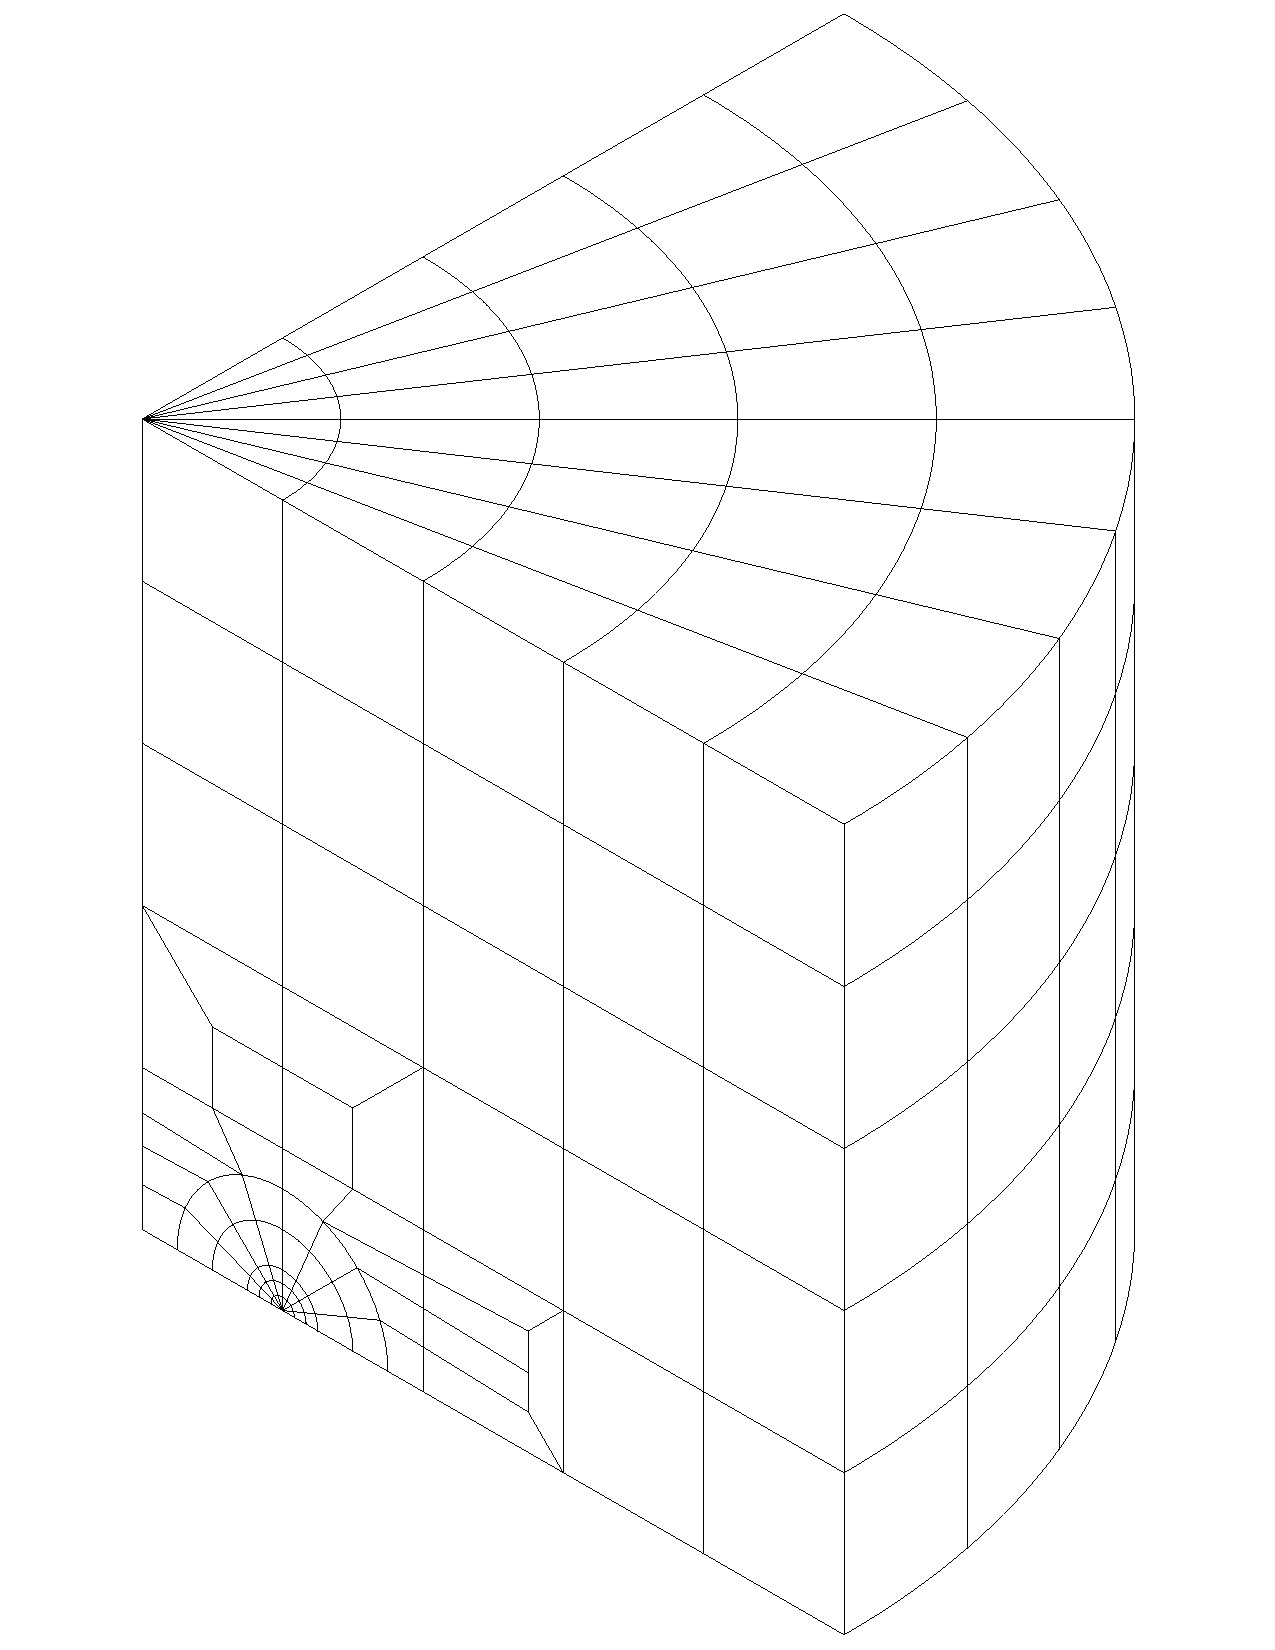
\includegraphics[width=0.5\columnwidth]{3d_body_mesh}
   \caption{Specimen model for embedded circular crack}
   \label{fig:specimen_model}
\end{figure}
\begin{figure}[tbp]
\centering
	   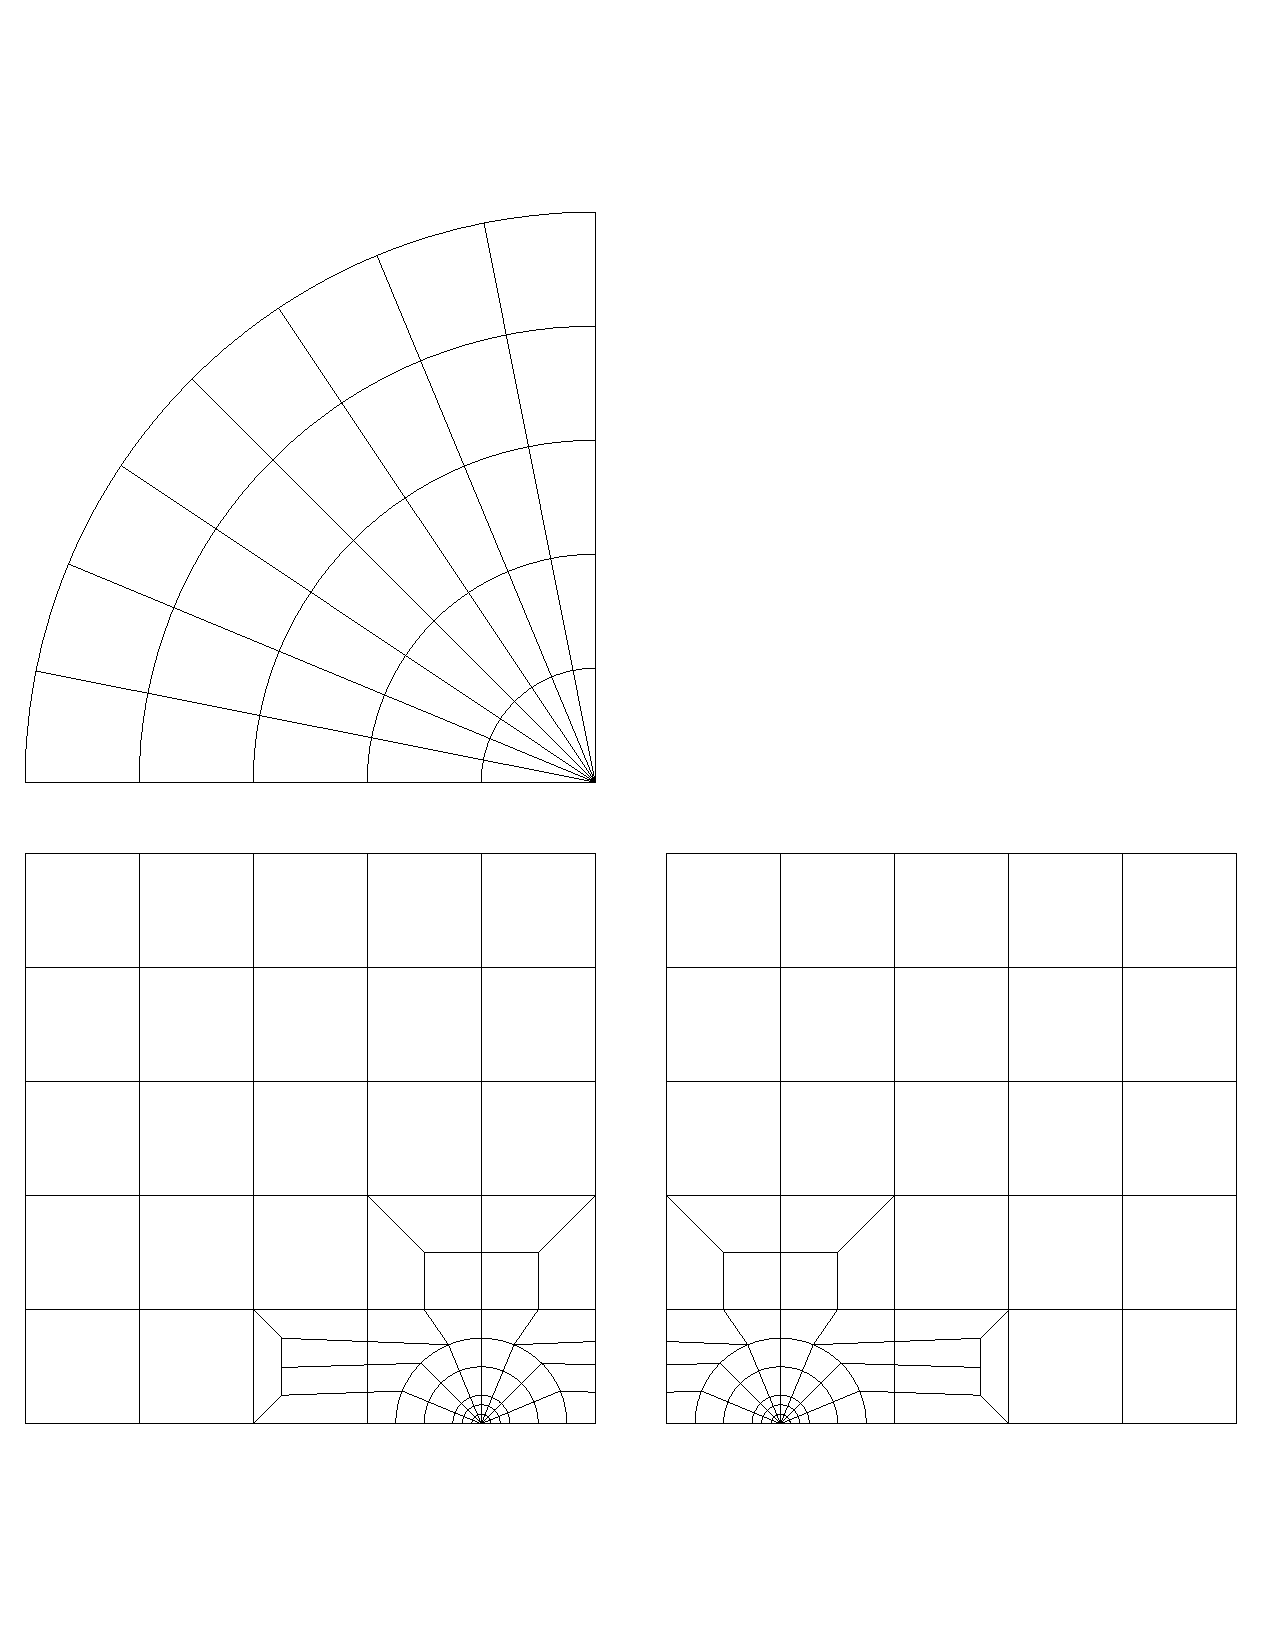
\includegraphics[width=0.7\columnwidth]{body_mesh_8segments}
      \caption{Orthographic views for specimen model for embedded circular crack}
      \label{fig:body_mesh_orthographic}
\end{figure}

One complicating feature of the elliptical crack models was their coordinate transformation from the circular crack front's $(x,y,z)$ Cartesian coordinates to a corresponding $(x',y',z')$ coordinate system shown in Figure~\ref{fig:circle_to_ellipse}. The coordinate transformation from $(x,y,z)$ to $(x',y',z')$ for $x$ and $z$ away from the origin is given by
\begin{align}
  x' &= x \sqrt{1+\frac{c^2-a^2}{x^2+z^2}} \\
  y' &= y \\
  z' &= z
\end{align}
for $\frac{a}{c} \leq 1$ and
\begin{align}
  x' &= x \\
  y' &= y \\
  z' &= z \sqrt{1+\frac{a^2-c^2}{x^2+z^2}}
\end{align}
for $\frac{a}{c} > 1$. Since these equations are invalid at the $(x,z)$ origin, the authors created a tiny cylindrical surface of radius $0.001 a$ around the origin. This surface was transformed into an very narrow, nearly flat ellipse on the elliptical surface-crack model shown in \Cref{fig:elliptical_model}.
\begin{figure}[tbp]
\centering
	   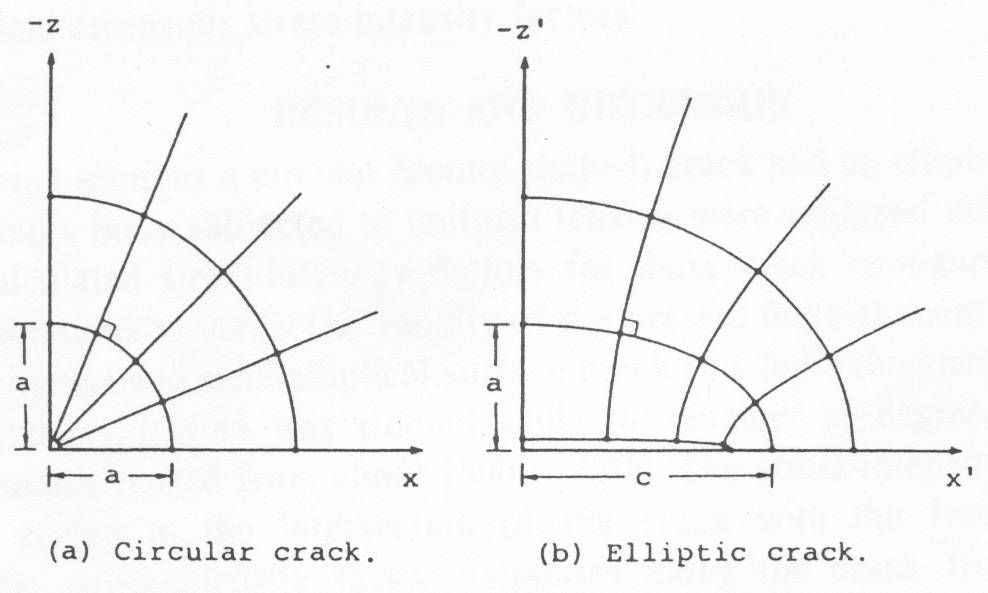
\includegraphics[width=0.8\columnwidth]{newman-raju-figure-3}
      \caption[Circle to ellipse transformation]{Circle to ellipse transformation \citep{rajunewman1979}}
      \label{fig:circle_to_ellipse}
\end{figure}
\begin{figure}[tbp]
\centering
	   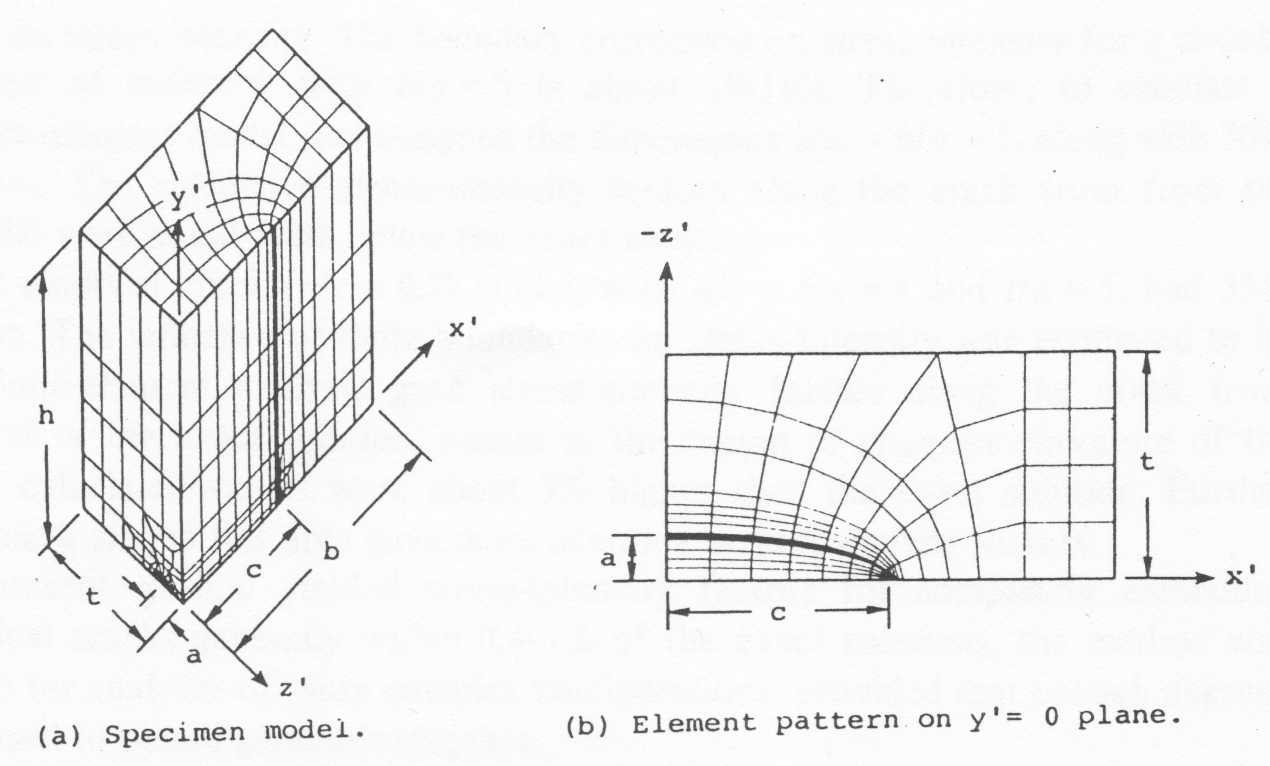
\includegraphics[width=0.8\columnwidth]{newman-raju-figure-4}
      \caption[Finite-element mesh for a semi-ellip\-tical surface crack]{Finite-element mesh for a semi-ellip\-tical surface crack \citep{rajunewman1979}}
      \label{fig:elliptical_model}
\end{figure}

All the models analyzed were in uniaxial tension with no shear stress, so only Mode I stress intensity factors are considered. The stress intensity factor $K$ is given by
\begin{align}
K &= \KI = \St \sqrt{\left( \pi \frac{a}{Q}\right) F\left(\frac{a}{t},\frac{a}{c},\phi\right)}
\end{align}
where \(Q\) is defined in \Cref{eq:shape-factor} and $F$\nomenclature[1F]{\(F\)}{Newman-Raju bound\-ary-cor\-rec\-tion factor} is an as-yet undefined bound\-ary-cor\-rec\-tion factor which is a function of the crack's depth, length, the plate's thickness, and the parametric angle of the ellipse.

The stress intensity factors for each model were calculated using a nodal-force method, removing the need to assume plane stress or plane strain conditions. This method was first developed by Raju and Newman in 1977, and summed nodal forces from the finite-element solution within a given radius $r$ and along the boundary between wedges $i$ and $i+1$ shown in Figure~\ref{fig:nodal_force_method} to calculate a series of apparent stress intensity factors $K_{\textnormal{ap}}$.  This force sum $F_y$ was given by
\begin{equation}
F_y = F_1 + F_2 + F_3 + \cdots + F_{j-1} + F'_{j}
\end{equation}
where there are $j$ nodes between the crack front and radius $r$. $F'_{j}$ is a modified nodal force at node $j$, excluding contributions from elements outside the radius $r$. This $F_y$ is substituted into
\begin{equation}
F_y = \frac{K_\textnormal{ap}}{\sqrt{2\pi}} \sqrt{2 r t_\textnormal{a}}
\end{equation}
where $t_\textnormal{a}$ is the average width of the singular elements on either side of $\phi$. Since $K_\textnormal{ap}$ is linear with respect to $r$ except at the crack front, a linear least-squares fit was applied to estimate $K_\textnormal{ap}$ at $r=0$. Note that this \(K_\textnormal{ap}\) is different than the apparent stress intensity factor \(K_\textnormal{Iapp}\) given in \Cref{eq:kiapp}.
\begin{figure}[tbp]
\centering
	   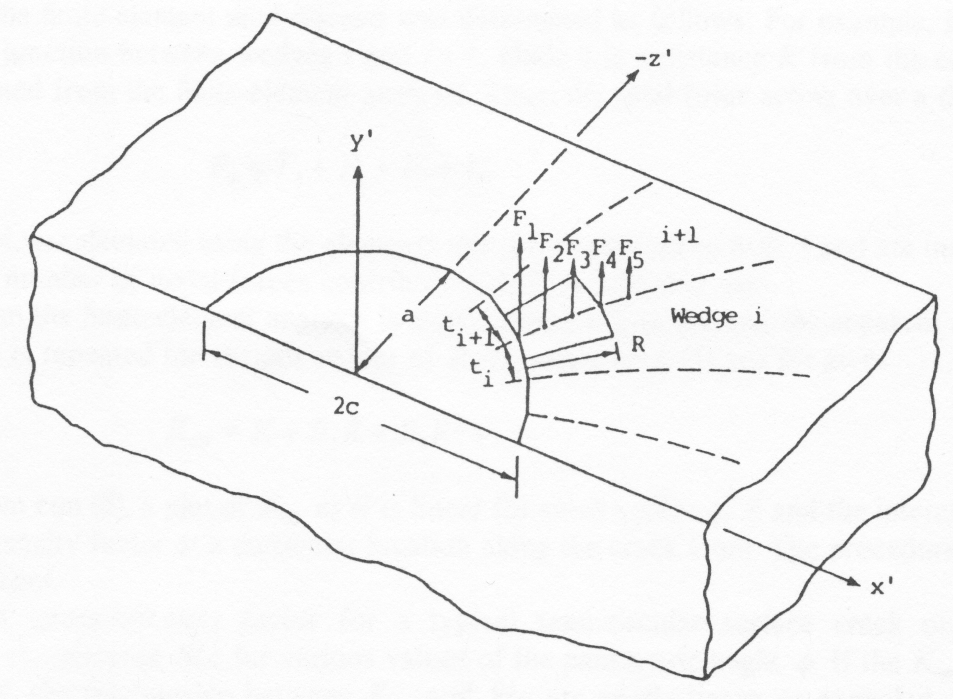
\includegraphics[width=0.8\columnwidth]{newman-raju-figure-13}
      \caption[Nodal forces on $y'=0$ plane and at the junction of wedges $i$ and $i+1$]{Nodal forces on $y'=0$ plane and at the junction of wedges $i$ and $i+1$ \citep{rajunewman1979}}
      \label{fig:nodal_force_method}
\end{figure}

The first group of results examined were for embedded circular (penny-shaped) cracks and embedded elliptical cracks. Both cracks were embedded in large bodies subjected to uniform tension. Exact solutions exist for both of these cases, so they were used to establish the validity of the finite element models, element types, and mesh sizing.

\citet{tadaparisirwin1973} demonstrated that the free surfaces of sufficiently large bodies have negligible effects on stress intensities in a crack compared to infinite bodies. For example, a body with dimensions five times larger than the crack dimensions only caused a 1\% difference in stress intensity factors. A circular crack embedded in a cylindrical body with 3078 degrees of freedom displayed stress intensity factors within 0.4\% of the exact solution.

For a narrow elliptical crack ($\frac{a}{c}=0.2$) in a large rectangular body, a finite element mesh with 3348 degrees of freedom gave results within 1\% of the exact values, except in regions where the ellipse had its greatest curvature. In those regions, the accuracy was around 3\%. Refining the mesh so that the elements were sized proportionally to the ellipse curvature improved the results to around 1\% of the exact values at all locations.

Mesh topologies from the $\phi=\frac{\pi}{2}$ plane were used to model a plane strain flat plate with a through-the-thickness crack.
The meshes from deeper cracks were used for models where the crack length $c$ was large compared to the plate half-width \(W\), and meshes from shallower cracks were used for models where the crack length was comparatively small.
For $0.2 \leq \frac{c}{W} \leq 0.6$, stress intensity factors were within 1.3\% of solutions from \citeauthor{tadaparisirwin1973}
For $\frac{c}{W} = 0.8$, stress intensity factors were 2\% lower.
Since the free boundaries of the idealized plate were very close to the crack front in the $\frac{c}{W}=0.8$ case, these results indicate that there are enough degrees of freedom in the mesh topology to accurately model the influence of the free surfaces in a three-dimensional model.

Now that the mesh in $R$ and $z$ directions was demonstrated to be sufficiently accurate, the authors investigated how many radial divisions the three-dimensional model should have. If the mesh had enough elements around the $\phi$ dimension, it should be able to accurately model stress intensity changes across the crack front and indicate where the worst stress intensity occurs.
As shown in Figure~\ref{fig:circular_convergence}, the authors plotted stress intensity versus $\phi$ for a circular surface crack in a rectangular body using 3 data points (2 mesh divisions with $\Delta \phi=45^\circ$), 5 data points ($\Delta \phi=22.5^\circ$), 9 data points ($\Delta \phi=11.25^\circ$), and 13 data points ($\Delta \phi=7.5^\circ$). The results for the two finest meshes were within 1\% of each other, indicating that the mesh with 8 divisions was sufficient to model stress intensity distribution along the crack front. The process was repeated for an elliptical surface crack in a rectangular body with similar results shown in Figure~\ref{fig:elliptical_convergence}.
\begin{figure}[tbp]
\centering
	   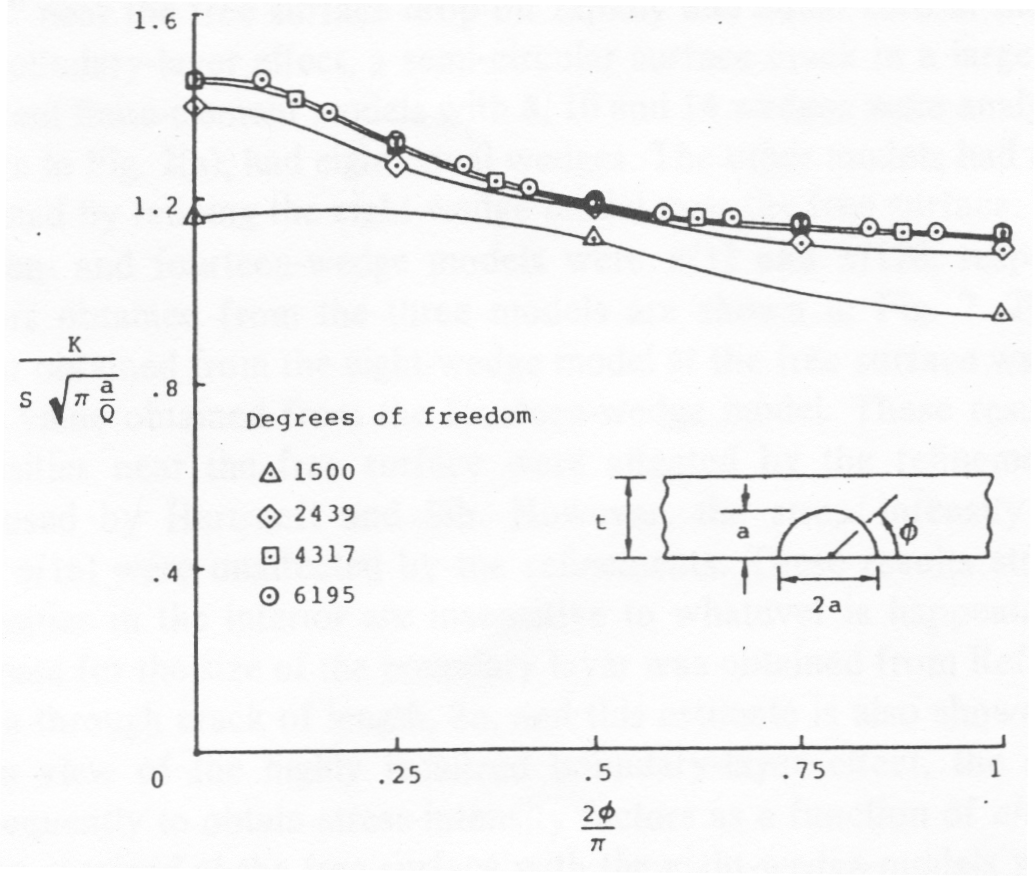
\includegraphics[width=0.8\columnwidth]{newman-raju-figure-5}
      \caption[Convergence of bound\-ary-cor\-rec\-tion factors for a deep semi-circu\-lar surface crack ($Q=\frac{\pi^2}{4}$, $\frac{a}{t}=0.8$)]{Convergence of bound\-ary-cor\-rec\-tion factors for a deep semi-circu\-lar surface crack ($Q=\frac{\pi^2}{4}$, $\frac{a}{t}=0.8$) \citep{rajunewman1979}}
      \label{fig:circular_convergence}
\end{figure}

\begin{figure}[tbp]
\centering
	   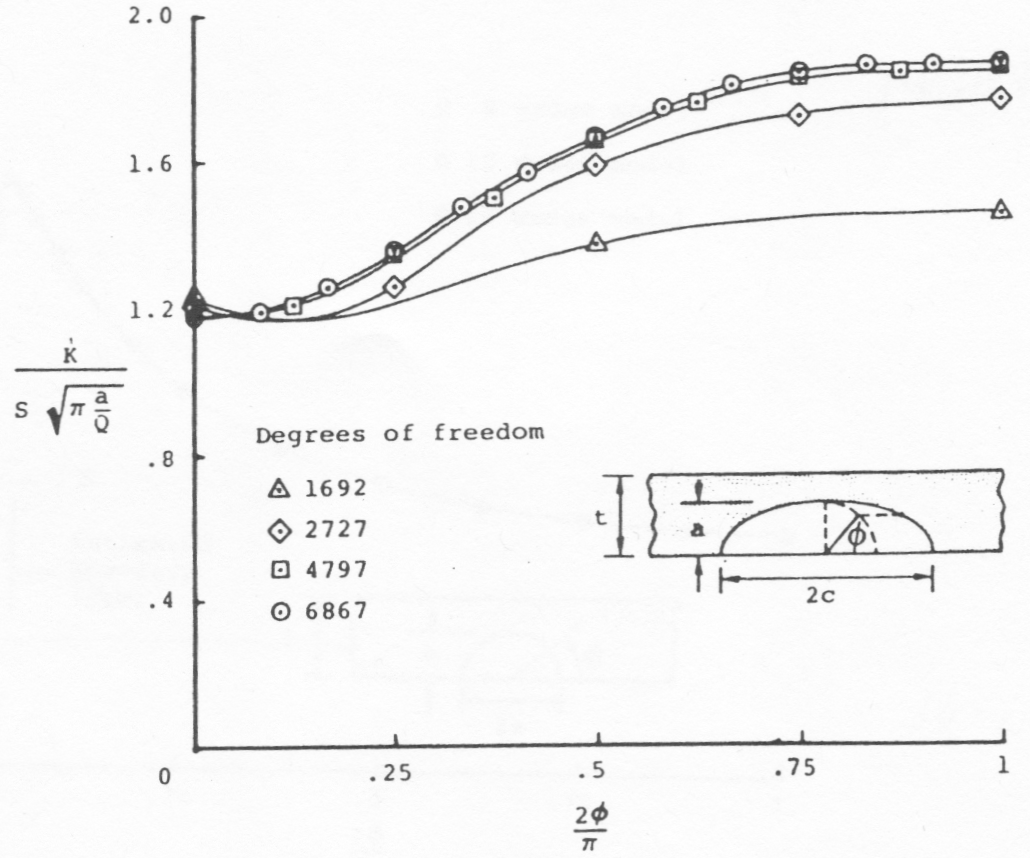
\includegraphics[width=0.8\columnwidth]{newman-raju-figure-6}
      \caption[Convergence of bound\-ary-cor\-rec\-tion factors for a deep semi-ellip\-tical surface crack ($Q=1.104$, $\frac{a}{t}=0.8$, $\frac{a}{c}=0.2$)]{Convergence of bound\-ary-cor\-rec\-tion factors for a deep semi-ellip\-tical surface crack ($Q=1.104$, $\frac{a}{t}=0.8$, $\frac{a}{c}=0.2$) \citep{rajunewman1979}}
      \label{fig:elliptical_convergence}
\end{figure}

\citet{hartranftsih1970} reported that stress intensity factors on plates with through cracks dropped rapidly toward zero at a free surface, and are exactly zero at the free surface itself.
And the finite element models used to create Figures~\ref{fig:circular_convergence} and \ref{fig:elliptical_convergence} have their worst convergence at and near the free surface.
Newman and Raju decided to refine their meshes at the free boundary to see if their models confirmed the bound\-ary-layer effect reported by Hartranft and Sih.
\begin{figure}[tbp]
\centering
	   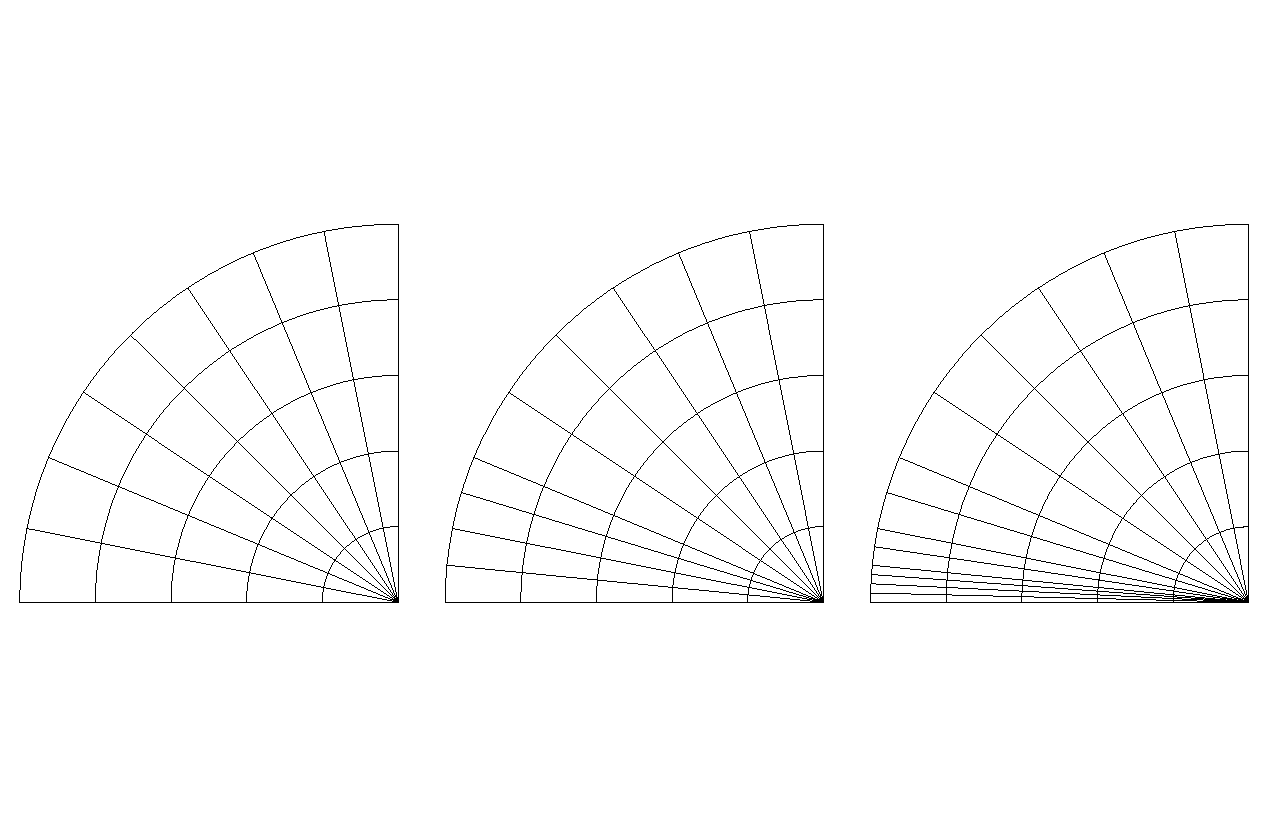
\includegraphics[width=\columnwidth]{3_meshes}
      \caption{Comparison of wedge sizes used in estimating bound\-ary-layer effect}
      \label{fig:wedge_refinement}
\end{figure}

They began with the model with eight equal wedges, and gradually refined the mesh near the free surface as shown in Figure~\ref{fig:wedge_refinement}.
The 10-wedge model had a minimum wedge angle of $\frac{\pi}{32}$, and the 14-wedge model had a minimum wedge angle of $\frac{\pi}{128}$.
Results for this are shown in Figure~\ref{fig:effects_of_mesh_refinement}.
Newman and Raju's finer-meshed models showed the stress intensity factor rising toward the free surface, and then falling off.
In the case of the 14-wedge model, the drop was much sharper than for the 10-wedge model.
This indicated that their models were able to account for Hartranft and Sih's bound\-ary-layer effect, and exhibited a boundary layer that was approximately the same size.
At $\phi>\frac{\pi}{16}$ away from the free surface, the stress intensity factors were unchanged from the models with a coarser mesh.
For the remainder of the models where the distribution of stress intensity factors across $\phi$ was examined, any stress intensity factor at the free surface should be read as an average stress intensity factor \emph{near} the free surface.
\begin{figure}[tbp]
\centering
	   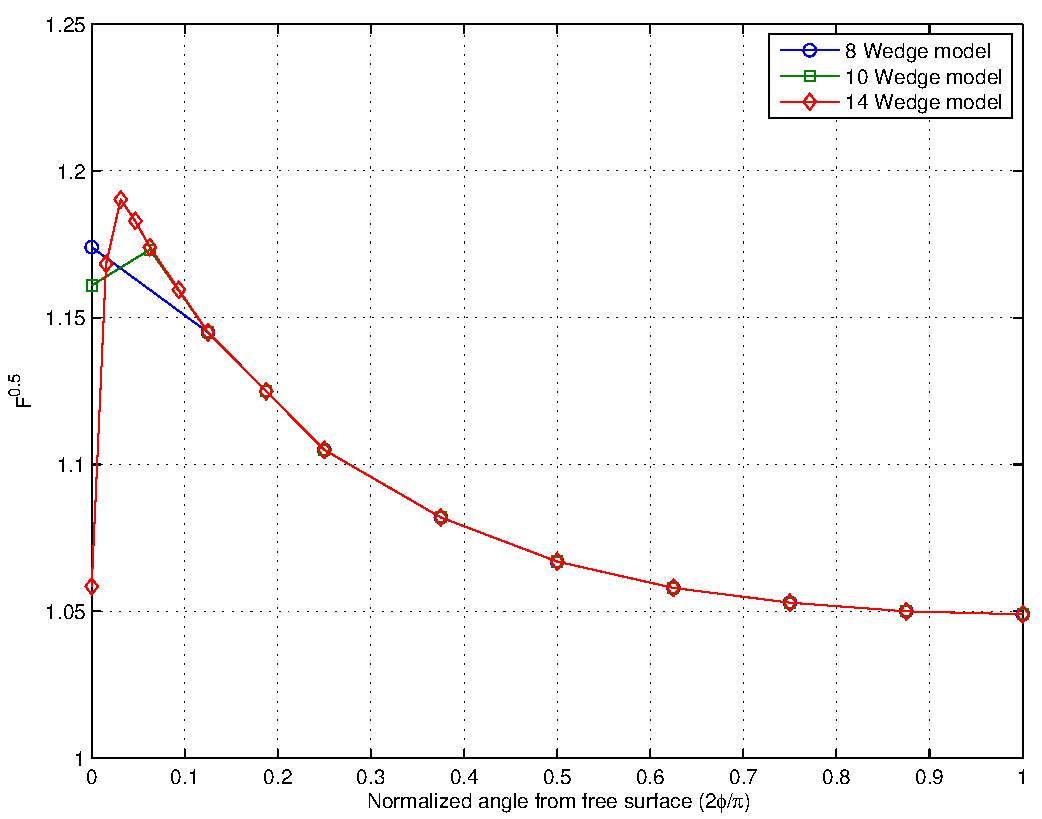
\includegraphics[width=0.6\columnwidth]{nr_fig7}
      \caption{Effects of mesh refinement near the free surface on the distribution of bound\-ary-cor\-rec\-tion factors for semi-circu\-lar surface crack ($Q=\frac{\pi^2}{4}$; $\frac{a}{t}=0.2$)}
      \label{fig:effects_of_mesh_refinement}
\end{figure}

The distribution of stress intensity factors along a crack front for various sizes of semi-circular surface cracks can be seen in Figure~\ref{fig:sif_circular}.
For shallow cracks, the stress intensity factor varied little across the crack front.
As the cracks grew deeper compared to the plate thickness, larger variations in stress intensity become apparent.
In all semi-circular crack sizes, the highest stress intensity factor occurred near the free surface.
\begin{figure}[tbp]
\centering
	   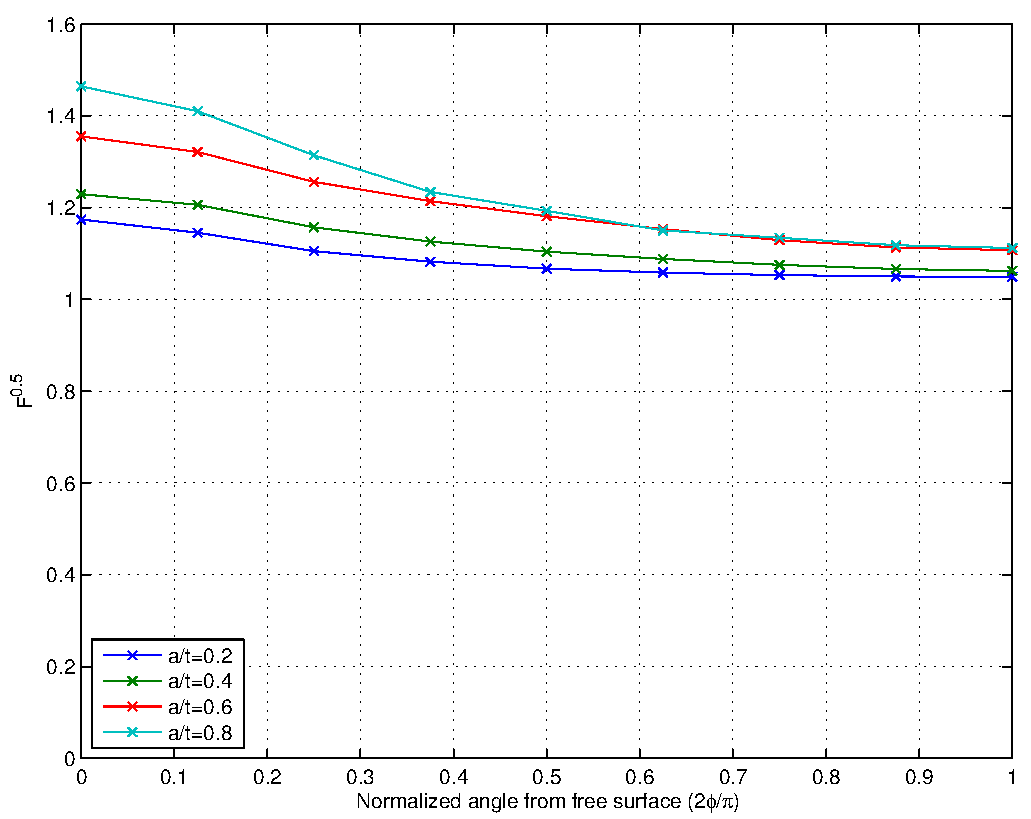
\includegraphics[width=0.6\columnwidth]{nr_fig8}
      \caption{Distribution of bound\-ary-cor\-rec\-tion factors along crack front for a semi-circu\-lar surface crack ($Q=\frac{\pi^2}{4}$)}
      \label{fig:sif_circular}
\end{figure}

The distribution of stress intensity factors along a crack front for various sizes of wide semi-elliptical surface cracks can be seen in Figure~\ref{fig:sif_02_ellipse}. In all the wide semi-elliptical crack sizes, the highest stress intensity factor occurred deep within the rectangular body.
\begin{figure}[tbp]
\centering
	   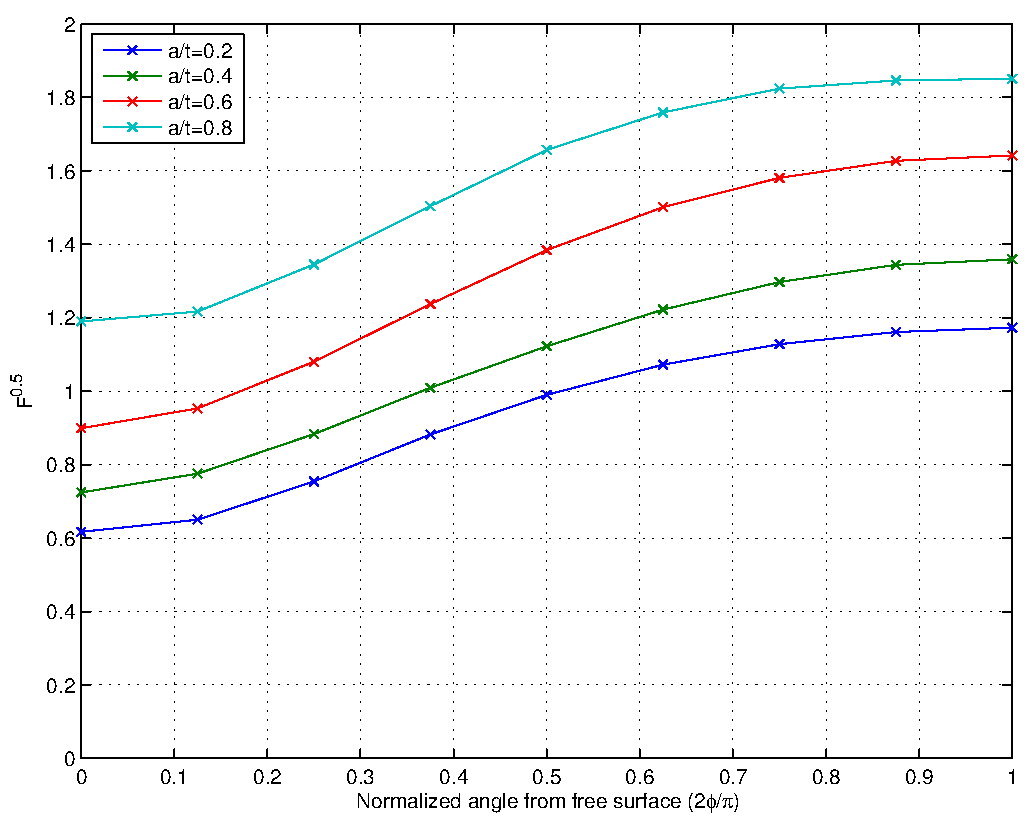
\includegraphics[width=0.6\columnwidth]{nr_fig9}
      \caption{Distribution of bound\-ary-cor\-rec\-tion factors along crack front for a semi-ellip\-tical surface crack ($Q=1.104$, $\frac{a}{c}=0.2$)}
      \label{fig:sif_02_ellipse}
\end{figure}
For deep semi-elliptical surface cracks ($\frac{a}{t}=0.8$) shown in Figure~\ref{fig:sif_08_thickness}, stress intensity factors were highest in the interior of the plate for relatively narrow cracks ($\frac{a}{c} \leq 0.4$), but highest near the free surface for wide cracks ($\frac{a}{c} \geq 1.0$).
\begin{figure}[tbp]
\centering
	   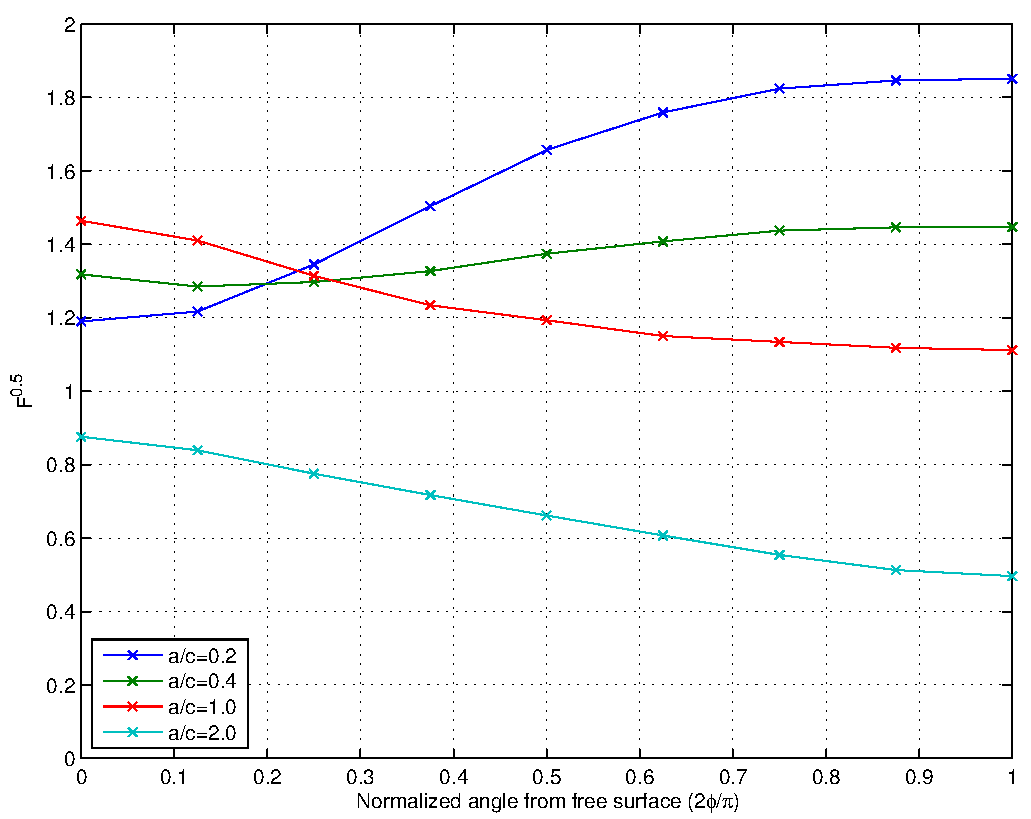
\includegraphics[width=0.6\columnwidth]{nr_fig10}
      \caption{Distribution of bound\-ary-cor\-rec\-tion factors along crack front for a semi-ellip\-tical surface crack ($\frac{a}{t}=0.8$)}
      \label{fig:sif_08_thickness}
\end{figure}

Figures~\ref{fig:prior_research_1} and \ref{fig:prior_research} show a comparison of Newman and Raju's results for deep semi-elliptical surface cracks against previously-published literature, and considerable differences are obvious.
Smith and Sor\-en\-sen's alternating method results matched the basic distribution of stress intensity factors, but their actual values were anywhere from 10--25\% lower than Raju and Newman's.
Kobayashi's alternating method was also similar in distribution, but showed even lower values than Sorensen, as much as 50\%.
Kathiresan's finite-element model matched the Raju-Newman model at the free surface, but its general distribution of stress intensity factors across the crack front varied greatly, and showed an erroneous minimal value at $\phi=45^\circ$.
A line-spring model developed by \citet{ricelevy1970} was within 3.5\% of the Raju-Newman model for $0.2 \leq \frac{a}{t} \leq 0.6$, but had an erroneous drop in stress intensity for $\frac{a}{t}=0.8$.
An earlier equation from \citet{newman1973} matched the finite-element results to within 5\% for $0.2 \leq \frac{a}{t} \leq 0.8$.
\begin{figure}[tbp]
\centering
	   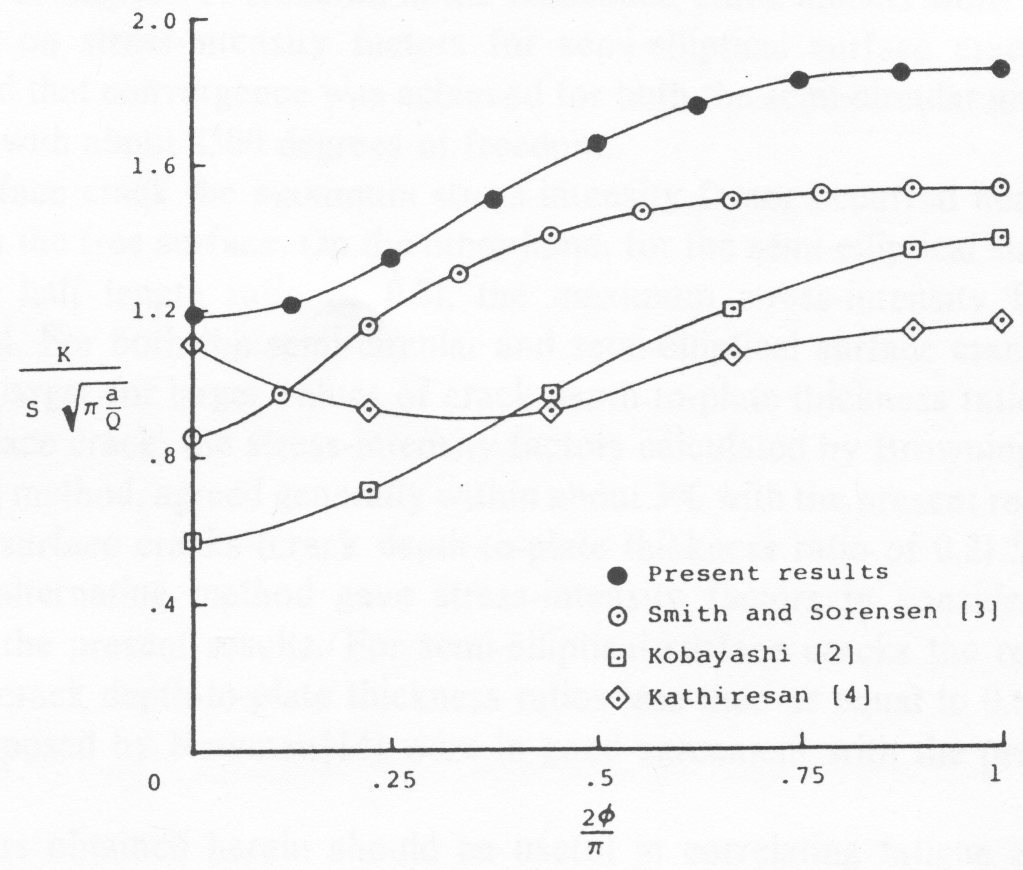
\includegraphics[width=0.6\columnwidth]{nr_fig11}
      \caption[Comparison of bound\-ary-cor\-rec\-tion factors for a deep semi-ellip\-tical surface crack ($Q=1.104$, $\frac{a}{t}=0.8$, $\frac{a}{c}=0.2$)]{Comparison of bound\-ary-cor\-rec\-tion factors for a deep semi-ellip\-tical surface crack ($Q=1.104$, $\frac{a}{t}=0.8$, $\frac{a}{c}=0.2$) \citep{rajunewman1979}}
      \label{fig:prior_research_1}
\end{figure}
\begin{figure}[tbp]
\centering
	   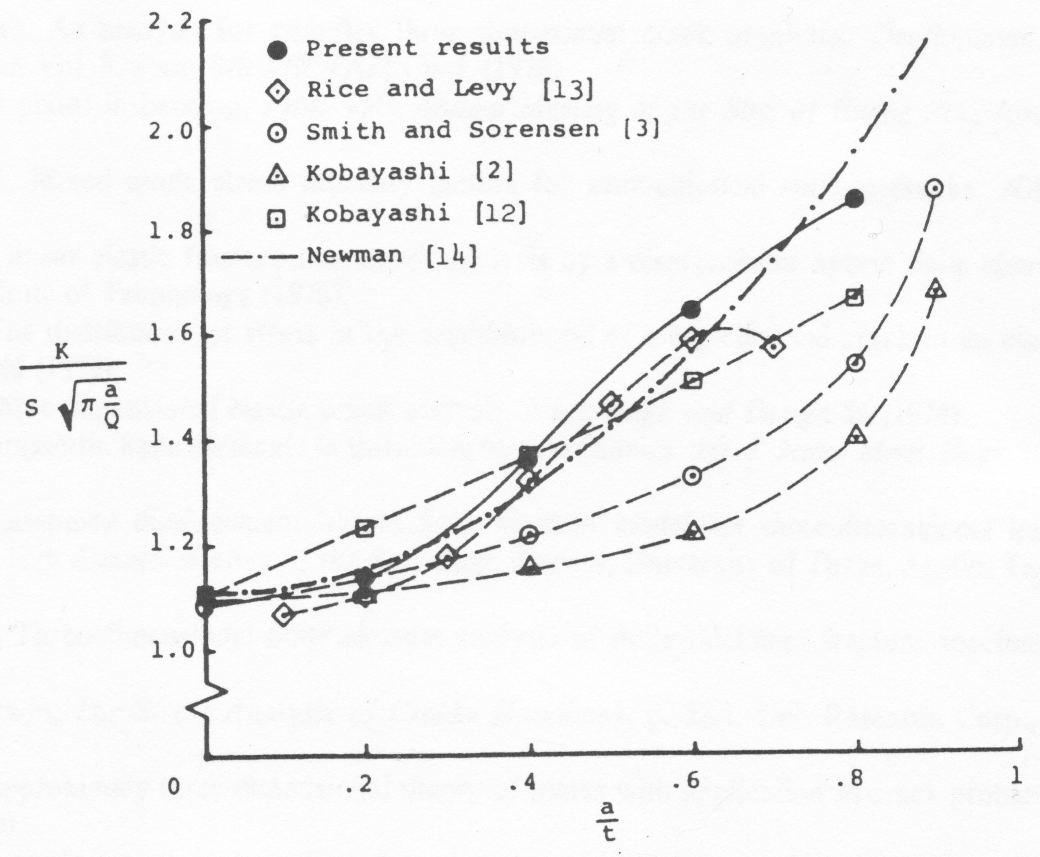
\includegraphics[width=0.7\columnwidth]{nr_fig12}
      \caption[Comparison of the maximum bound\-ary-cor\-rec\-tion factor for a semi-ellip\-tical surface crack as a function of $\frac{a}{t}$ ($\phi=\frac{\pi}{2}$, $Q=1.104$, $\frac{a}{c}=0.2$)]{Comparison of the maximum bound\-ary-cor\-rec\-tion factor for a semi-ellip\-tical surface crack as a function of $\frac{a}{t}$ ($\phi=\frac{\pi}{2}$, $Q=1.104$, $\frac{a}{c}=0.2$) \citep{rajunewman1979}}
      \label{fig:prior_research}
\end{figure}

The boundary-correction factor \(F\) was curve-fitted, and the mode I stress intensity factor \KI for any point along the crack front \((x_\textnormal{e}, y_\textnormal{e})\) was reformatted as
\begin{align}
\KI &= \St \sqrt{F\left(\frac{a}{t},\frac{a}{c},\phi\right) \left( \pi \frac{a}{Q}\right)}.
\end{align}

\subsection{Elastic-Plastic Fracture}

Just as Irwin extended Griffith's theories of brittle fracture to include the effects of small-scale yielding near the crack tip, \citet{wells1961} extended Irwin's theories to account for larger-scale yielding and materials with much higher fracture toughness.
While attempting to characterize critical stress intensity values (\KIc) for extremely tough structural steel alloys, Wells noticed the crack faces moved apart before fracture, changing an originally sharp crack into a more blunt shape.
This led Wells to correlate fracture toughness with the size of the opening at the crack tip, now known as the crack tip opening displacement (CTOD\nomenclature[1CTOD]{CTOD}{crack tip opening displacement} or \(\deltat\)\nomenclature[2\deltat]{\(\deltat\)}{crack tip opening displacement (identical to CTOD)}).

One estimate for CTOD uses linear elastic equations for the displacement field at a position \ry behind the tip of a crack with effective length \(a+\ry\) shown in \Cref{fig:ctod-irwin}:
\begin{figure}[tbp]
\centering
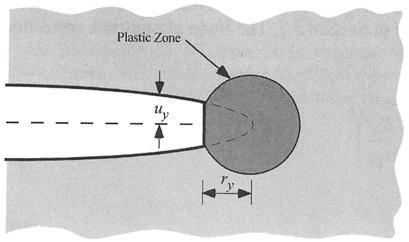
\includegraphics{ctod-irwin}
\caption[Estimation of CTOD from displacement field of crack with Irwin plastic radius correction]{\label{fig:ctod-irwin} Estimation of CTOD from displacement field of crack with Irwin plastic radius correction \citep{anderson2005}}
\end{figure}
\begin{align}
\deltat &= 2 u_{y} = \frac{8}{E'} \KI \sqrt{\frac{\ry}{2\pi}} . \label{eq:ctod-irwin}
\end{align}

One goal of elastic-plastic fracture theory is the extension of linear elasticity theories to a more general, nonlinear elasticity known as deformation plasticity theory.
The nonlinear equivalent to the linear elastic strain energy release rate \G is \J,\nomenclature[1J]{\J}{elastic-plastic fracture parameter} which can be defined in terms of a contour integral surrounding the crack tip as shown in \Cref{fig:contour-integral}.
\begin{figure}[tbp]
\centering
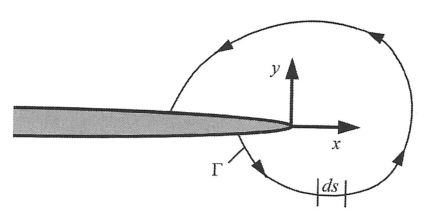
\includegraphics[width=0.5\columnwidth]{contour-integral}
\caption[Path-independent contour integral surrounding a crack tip]{\label{fig:contour-integral} Path-independent contour integral surrounding a crack tip \citep{anderson2005}}
\end{figure}
For the counterclockwise contour path \(\Gamma\) shown,
\begin{align}
\J &= \int_{\Gamma} \left( w \, {dy} - T_i \pderiv{u_i}{x} \, {ds}\right) \label{eq:j-contour-integral}
\end{align}
where
\begin{align*}
w &= \textnormal{strain energy density} \nomenclature[1w]{\(w\)}{strain energy density} \\
T_i &= \textnormal{components of traction vector} \nomenclature[1Ti]{\(T_i\)}{components of traction vector} \\
u_i &= \textnormal{components of displacement vector} \nomenclature[1ui]{\(u_i\)}{components of displacement}\\
ds &= \textnormal{differential length along \(\Gamma\)}
\end{align*}
The strain energy density \(w\) and traction vector \(T_i\) are related to the stress and strain fields by
\begin{align}
w &= \Int{\sigma_{ij}}{\epsilon_{ij},0,\epsilon_{ij}} \\
T_i &= \sigma_{ij} n_j
\end{align}
where \(\sigma_{ij}\)\nomenclature[2\sigma_ij]{\(\sigma_{ij}\)}{stress tensor} and \(\epsilon_{ij}\)\nomenclature[2\epsilon]{\(\epsilon_{ij}\)}{strain tensor} are the stress and strain tensors, and \(n_j\)\nomenclature[1n]{\(n_j\)}{components of vector normal to contour path} are the components of a vector normal to the contour path.
\citet{rice1968} demonstrated that the contour integral version of \J was constant for any chosen path \(\Gamma\).
In other words, \J is a path-independent integral.

Alternatively, \J can be defined in terms of a nonlinear strain energy release rate
by \cite{rice1968} as
\begin{align}
J &= - \D{\Pi}{A}
\intertext{where}
dA &=
  \begin{cases}
  t \,da & \textnormal{for an edge-cracked plate} \\
  2 t \,da & \textnormal{for a center-cracked plate} \\
  2\pi a \,da & \textnormal{for an embedded circular crack}
  \end{cases}
\intertext{and}
\Pi &= U - F
\end{align}
where \(U\)\nomenclature[1U]{\(U\)}{strain energy stored in a body} is the strain energy stored in the body and \(F\)\nomenclature[1F]{\(F\)}{work done by external loads} is the work done by the applied load \(P\)\nomenclature[1P]{\(P\)}{applied load}. An example of an edge-cracked plate with nonlinear material behavior is shown in \Cref{fig:nonlinear-energy-release-rate}.
\begin{figure}[tbp]
\centering
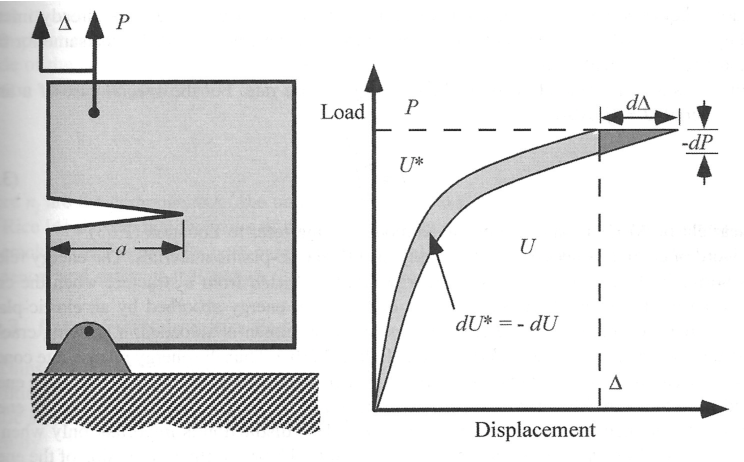
\includegraphics[width=\columnwidth]{nonlinear-energy-release-rate}
\caption[Nonlinear energy release rate]{\label{fig:nonlinear-energy-release-rate} Nonlinear energy release rate \citep{anderson2005}}
\end{figure}

The plate's strain energy at a given point on the load-dis\-place\-ment curve is
\begin{align}
U &= \Int{P}{\Delta,0,\Delta}
\end{align}
with \(\Delta\)\nomenclature[2\Delta]{\(\Delta\)}{load-line displacement of a plate} representing the load-line displacement of the plate.
The total potential energy \(\Pi\) for the plate under a constant load \(P\) is
\begin{align}
\Pi &= U - P \Delta = -U^{*}
\intertext{where}
U^{*} &= \Int{\Delta}{P,0,P}
\intertext{resulting in a strain energy release rate for a growing crack of}
J &= \left( \D{U^{*}}{A} \right)_{P} \\
  &= \Int{\left( \pderiv{\Delta}{A} \right)_{P}}{P,0,P} .
\end{align}
Similarly, for a plate held at a fixed displacement \(\Delta\), the external work \(F=0\) and the total potential energy \(\Pi=U\), resulting in a strain energy release rate of
\begin{align}
J &= - \left( \D{U}{A} \right)_{\Delta} \\
  &= - \Int{\left( \pderiv{P}{A} \right)_{\Delta}}{\Delta,0,\Delta} .
\end{align}
For the simpler case where the load-dis\-place\-ment response is linear, \J can be simplified as
\begin{align}
\J &= \Jel = \frac{\KI^2}{E'} = \G \label{eq:j-g} .
\end{align}

Finally, \J can be expressed in terms of a nonlinear stress intensity parameter, alluded to in \Cref{eq:j-g}.
\J provides a single-parameter characterization of stresses and strains for materials with significant plastic deformation near the crack tip.
Both \citet{hutchinson1968} and \citet{ricerosengren1968} used a Ramberg-Osgood power-law equation for a material's elastic-plastic stress-strain curve
\begin{equation}
\frac{\epsilon}{\epsilon_0} = \frac{\sigma}{\sigma_0} + \alpha \left( \frac{\sigma}{\sigma_0} \right)^{n}
\end{equation}
where
\begin{align*}
\sigma_0 &= \textnormal{reference stress value, often equal to yield strength} \\
\epsilon_0 &= \frac{\sigma_0}{E} \\
\alpha &= \textnormal{yield offset parameter, often 0.5} \\
n &= \textnormal{strain hardening exponent}
\end{align*}%
\nomenclature[2\sigma_0]{\(\sigma_0\)}{Ramberg-Osgood reference stress value, often equal to yield strength}%
\nomenclature[2\alpha]{\(\alpha\)}{Ramberg-Osgood yield offset parameter}%
\nomenclature[1n]{\(n\)}{Ramberg-Osgood strain hardening exponent}%
to calculate stresses and strains near a crack tip.
An example of this stress-strain curve is shown in \Cref{fig:ramberg-osgood}.
\begin{figure}[tbp]
\centering
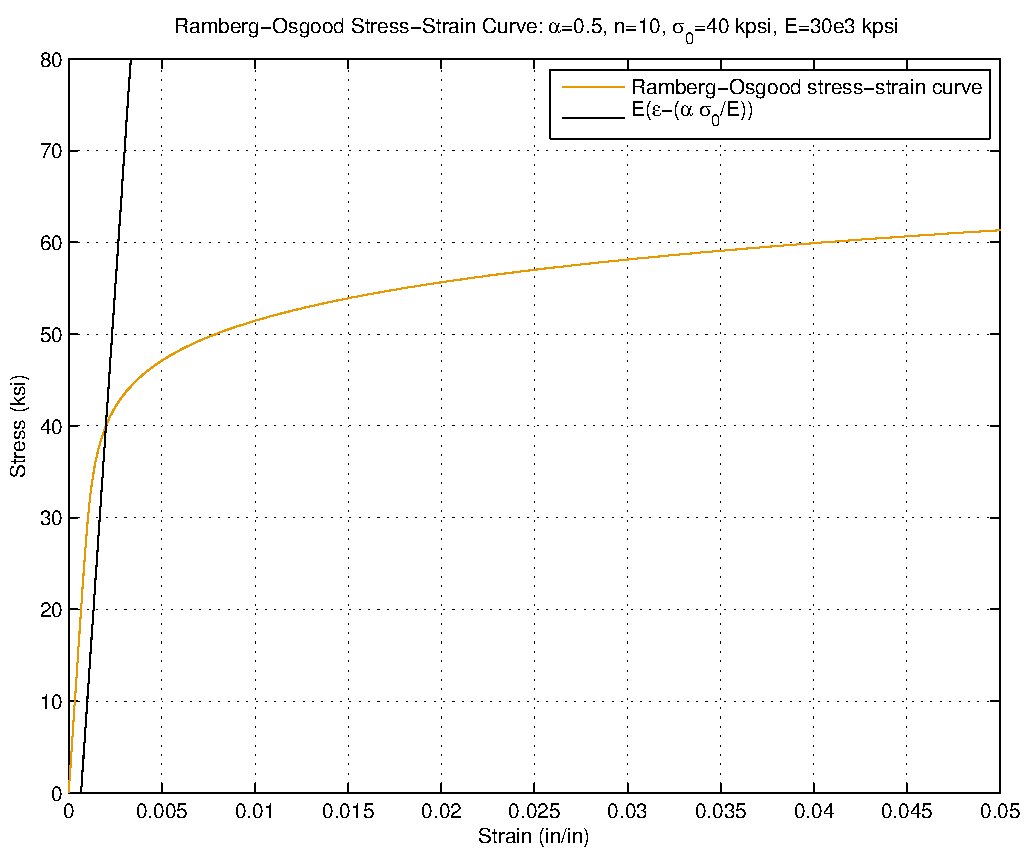
\includegraphics[width=0.8\columnwidth]{ramberg-osgood}
\caption{\label{fig:ramberg-osgood} Ramberg-Osgood stress strain curve}
\end{figure}
